\chapter{La jonction pn}
\label{ch:pnjunction}

%\section{Aperçu du chapitre}
Dans cette section, nous démontrons qu'une jonction formée entre un échantillon de semi-conducteur de type $p$ et un échantillon de type $n$ possède les propriétés d'un redresseur. Ce dispositif à deux bornes est appelé \emph{diode à jonction}. La structure physique et le symbole d'une jonction pn sont présentés dans la figure \ref{fig:pnjunction}.

\begin{figure}[h!]
\centering
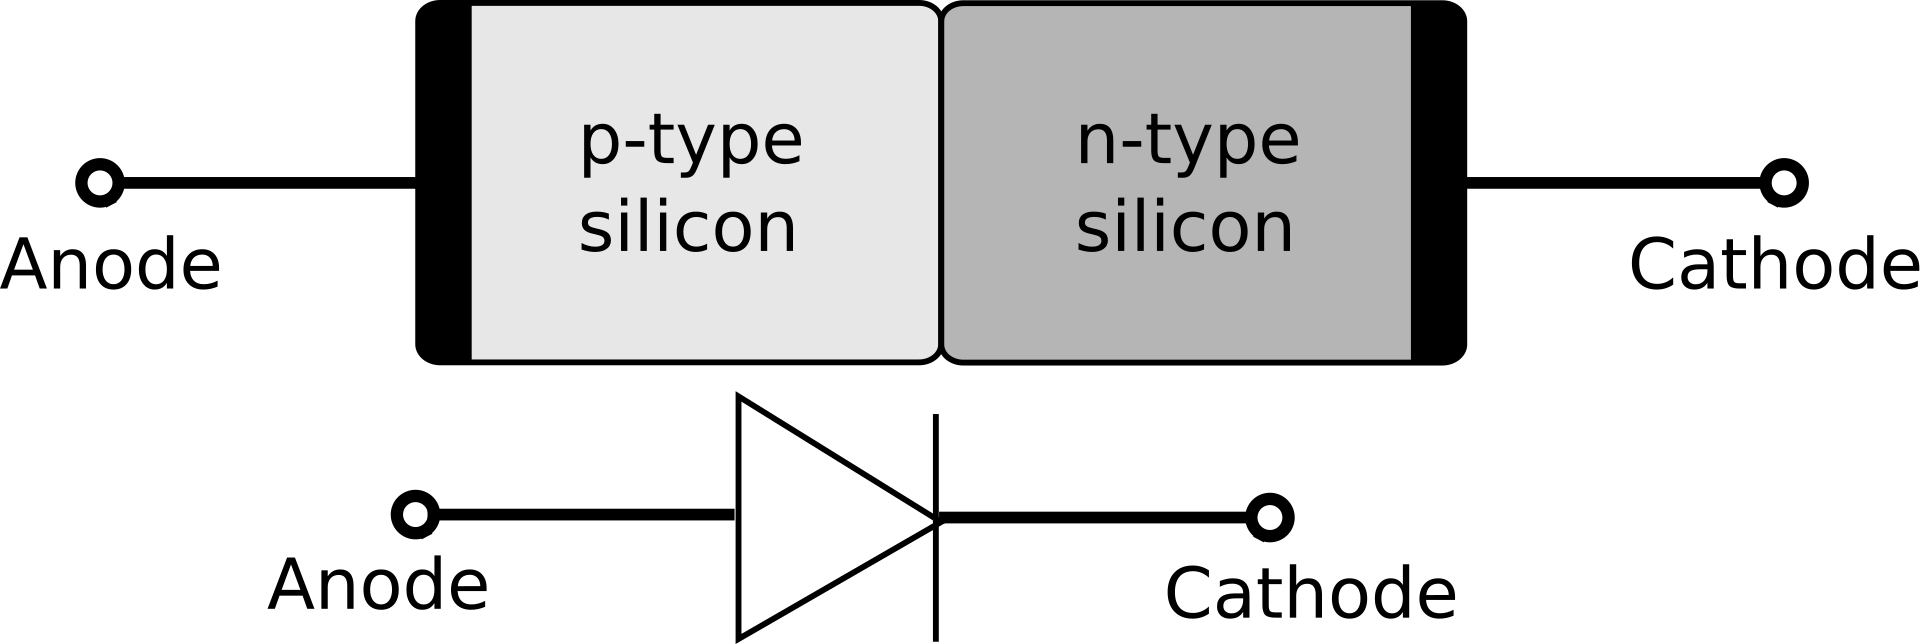
\includegraphics[width=12cm]{figures/ch01/pnjunction.png}
\caption{Structure (above) and symbol (below) of a pn-junction} 
\label{fig:pnjunction}
\end{figure}

Nous discuterons de la jonction en équilibre ainsi que sous polarisation directe et inverse. La caractéristique I-V sera dérivée et les concepts de la rupture de avalanche et de la capacité de déplétion seront abordés.

\section{La jonction pn en équilibre}
Si des impuretés donneuses sont introduites d'un côté et des accepteurs de l'autre côté d'un monocristal d'un semi-conducteur, une jonction $pn$ est formée\footnote{Ceci est appelé une jonction abrupte}. À l'interface, il y a par construction un gradient de concentration et donc des électrons et des trous diffuseront de chaque côté. Les électrons du type n se recombinent avec les trous majoritaires du type p et les trous du type p se recombinent avec les électrons majoritaires du type n. En conséquence, les ions dopants seront exposés et le côté n aura une densité de charge positive fixe ($N_d$) tandis que le côté p aura une densité de charge négative fixe ($N_a$) (figure \ref{fig:pn_equilibrium} (a)). Cette accumulation de charge entraînera un champ électrique interne pointant du type n vers le type p et agira donc contre tout courant de diffusion supplémentaire (\ref{fig:pn_equilibrium} (b)). Nous supposons pour le moment qu'aucune polarisation externe n'est appliquée, de sorte qu'aucun courant net ne peut circuler. La zone où les porteurs majoritaires ont diffusé et se sont recombinés est la \emph{zone de charge d'espace}\footnote{Également appelée la région de déplétion}. Pour préserver la neutralité de charge, nous exigeons que :
$$
N_A \; x_p = N_d \; x_n
$$
avec $x_p$ et $x_n$ la profondeur de la zone de charge d'espace dans le type p et n ($W_{Dp}$ et $W_{Dn}$ dans la figure \ref{fig:pn_equilibrium}). Comme on peut le déduire de cette expression, la zone de charge d'espace s'étend davantage dans le matériau faiblement dopé.\
Parce que $\frac{d\mathcal{E}}{dx} = \rho/\epsilon$, le champ électrique qui résulte de cette accumulation de charge est calculé comme $\mathcal{E}(x) = \int \rho(x)/\epsilon ; dx$ avec $\rho(x)$ le profil de charge local :
\begin{equation}
	\begin{split}
		\rho(x) &= -N_a \text{ si } x < 0 \\
		&= ; N_d \text{ si } x > 0
	\end{split}
\end{equation}
Le champ électrique maximum correspond à l'accumulation de charge totale et est négatif puisque le type p est placé à gauche : $|\mathcal{E}_m| = \epsilon N_a x_p = \epsilon N_d x_n$. Un champ électrique donne naissance à une différence de potentiel puisque $\mathcal{E} = -\frac{d\psi}{dx}$ comme dans la figure \ref{fig:pn_equilibrium}(c) où le soi-disant potentiel de jonction $\psi{bi}$ est égal à la surface sous $\mathcal{E}(x)$:
$$
\psi_{bi} = \frac{1}{2} (x_n + x_p) |\mathcal{E}_m| = \frac{1}{2} \epsilon (x_n + x_p)  N_a x_p
$$
Cette tension de jonction est également visible sur la figure \ref{fig:pn_equilibrium} (d) où les bandes d'énergie sont représentées. En raison du champ électrique, les bandes se courbent (dans la direction opposée à celle du potentiel, car $E=-qV$) à la jonction. Cette dernière figure est importante et peut également être construite en raisonnant avec les niveaux de Fermi. \
La largeur totale $W = x_n + x_p$ de la région de charge d'espace peut être calculée en fonction des niveaux de dopage et de la tension de jonction intrinsèque. Le résultat est :
\begin{equation}
    W = \sqrt{\frac{2 \epsilon}{q} \Big(\frac{N_a + N_d}{N_a N_d}\Big) V_{bi}}
    \label{eq:SCR_width}
\end{equation}

\begin{figure}[h!]
	\centering
	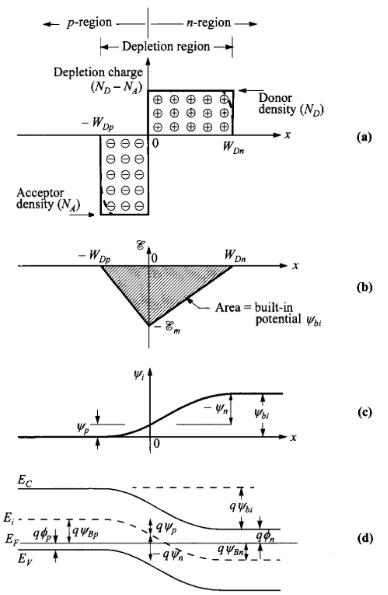
\includegraphics[width=8cm]{figures/ch01/pn_equilibrium.jpg}
	\caption{jonction pn en équilibre thermique}
	\label{fig:pn_equilibrium}
\end{figure}
\subsection{Niveaux de Fermi en équilibre}
Puisqu'aucun courant net ne peut circuler dans la jonction sans polarisation externe, le courant de dérive doit être égal au courant de diffusion. Pour les trous, cette condition donne:
\begin{equation}
    \begin{split}
       J_p  &= J_{p, drift} + J_{p, diffusion} \\
            &= q \mu_p p \mathcal{E} - q D_p \frac{dp}{dx} \\
            &= q \mu_p p \Big(\frac{1}{q} \frac{dE_i}{dx} \Big) - k T \mu_p \frac{dp}{dx}  = 0\\
    \end{split}
    \label{eq:jp_equilibrium}
\end{equation}
En équilibre, nous pouvons appliquer les équations de Boltzmann :
\begin{equation}
    p = n_i e^{(E_i - E_F)/kT}
    \label{eq:boltzmann_ch2}
\end{equation}
et calculer $\frac{dp}{dx}$ :
$$
\frac{dp}{dx} = \frac{p}{kT} \Big( \frac{dE_i}{dx} - \frac{dE_F}{dx} \Big)
$$
En substituant ceci dans l'équation \ref{eq:jp_equilibrium}, nous obtenons :
$$
J_p = \mu_p p \frac{dE_F}{dx} = 0 
$$
ou $\frac{dE_F}{dx} = 0$. Un résultat similaire est valable pour les électrons. \textbf{Pour qu'il y ait zéro courant net d'électrons et de trous, le niveau de Fermi doit être constant.}\\
Comme on peut le voir dans la figure \ref{fig:pn_equilibrium}(d), le niveau de Fermi $E_F$ reste constant le long de la jonction car il n'y a pas de courant net. Étant donné que $E_F$ est proche de $E_V$ dans le matériau de type p et proche de $E_C$ dans le matériau de type n, les bandes doivent se plier comme dans la figure pour maintenir un $E_F$ constant.

\subsection{Le potentiel de jonction intrinsèque}
Nous allons maintenant calculer $V_{bi} = \psi_n - \psi_p$ (précédemment noté $\psi_{bi}$). Nous savons qu'à distance de la jonction, il n'y a pas de charges nettes présentes, donc le potentiel doit obéir à l'équation de Laplace:
$$
\frac{d^2 \psi}{dx^2} = 0
$$
et $N_d - N_a + p - n = 0$ pour préserver la neutralité de charge. Dans un matériau de type p, nous supposons que $N_d = 0$ et $p \gg n$. Cela donne $p = N_a$. En insérant cela dans l'équation \ref{eq:boltzmann_ch2}, on obtient :
$$
\psi_p = -\frac{1}{q} (E_i - E_f) |_{x < x_p} = \frac{kT}{q} \ln\Big(\frac{N_a}{n_i}\Big)
$$
De même, le potentiel électrostatique pour le matériau de type n est
$$
\psi_n = -\frac{1}{q} (E_i - E_f) |_{x > x_n} = \frac{kT}{q} \ln\Big(\frac{N_d}{n_i}\Big)
$$
Le potentiel de jonction intrinsèque $V_{bi}$ est la différence de potentiel électrostatique entre le côté p et le côté n à l'équilibre thermique:
\begin{equation}
    V_{bi} = \psi_n - \psi_p = \frac{kT}{q} \ln\Big(\frac{N_a N_d}{n_i^2}\Big)
    \label{eq:vbi}
\end{equation}

\section{La jonction pn sous polarisation.}

\subsection{Polarisation directe}
Supposons que nous appliquons une tension positive $V_F$ à l'anode (côté p) tout en maintenant la cathode (côté n) à la masse. L'effet est que nous réduisons la barrière du potentiel intégré de $V_{bi}$ à $V_{bi}-V_F$, comme illustré sur le côté gauche de la figure \ref{fig:pn_bias}. Cela a plusieurs conséquences :
\begin{itemize}
	\item La largeur de la région de déplétion va diminuer, car l'équation \ref{eq:SCR_width} peut être réécrite comme :
	\begin{equation}
		W = \sqrt{\frac{2 \epsilon}{q} \frac{N_a + N_d}{N_a N_d} (V_{bi} - V_F)}
		\label{eq:SCR_width_bias}
	\end{equation}
	\item La valeur maximale de la $\mathcal{E}$  est réduite. Cela signifie qu'il y a un déséquilibre entre le courant de diffusion et le courant de dérive, et qu'il y aura un flux net (de diffusion) de trous du côté p vers le côté n et un flux d'électrons du côté n vers le côté p. Le résultat est un courant net du côté p vers le côté n.\footnote{Remarquez que les électrons peuvent diffuser de basse à haute énergie, alors qu'ils dérivent toujours de haute à basse énergie.}
\end{itemize}
Il y a donc un courant de diffusion de porteurs majoritaires à travers la région de déplétion vers l'autre côté, où ils deviennent les porteurs minoritaires. Comme il y a beaucoup de porteurs majoritaires disponibles, ce courant peut devenir très important lorsque la barrière de potentiel est suffisamment abaissée.\\
Remarquez également que les niveaux de Fermi dans la figure \ref{fig:pn_bias} ne sont plus constants, car il y a un courant et nous ne sommes plus en équilibre.

\begin{figure}[h!]
\centering
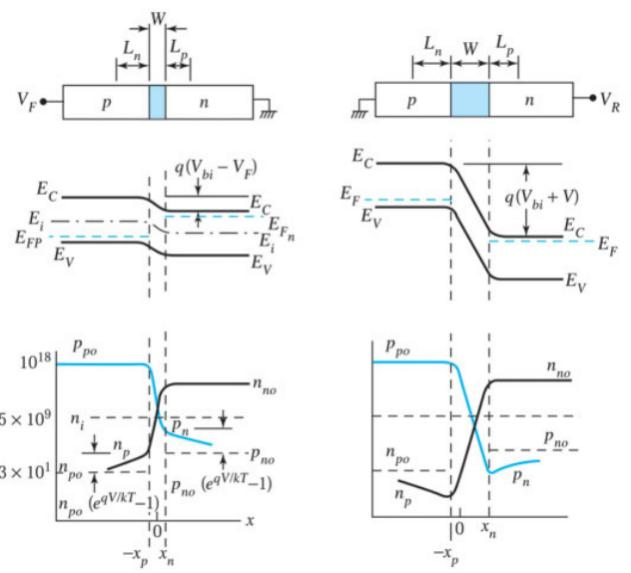
\includegraphics[width=12cm]{figures/ch01/pn_bias.jpg}
\caption{pn-junction under forward (left) and reverse (right) bias} 
\label{fig:pn_bias}
\end{figure}

\subsection{Polarisation inverse}
Lorsque nous appliquons une tension positive $V_R$ à la cathode (côté n) tout en gardant l'anode à la masse, nous augmentons la barrière du potentiel intégré à $V_{bi}+V_R$. Cette situation est esquissée à droite de la figure \ref{fig:pn_bias}. Selon l'équation \ref{eq:SCR_width_bias}, la largeur de la région de charge d'espace augmentera (parce que nous pouvons remplacer $V_F$ par $-V_R$). Le champ électrique interne au niveau de la jonction devient plus grand qu'avant, donc il peut y avoir un courant de dérive net. Cependant, les porteurs disponibles pour être balayés à travers la région de charge d'espace par le champ électrique sont les porteurs minoritaires des deux côtés de la jonction. Par conséquent, le courant résultant (le courant de saturation) sera très faible.

\subsection{Caractéristique de la diode}
Calculons les courants en supposant :
\begin{enumerate}
	\item que la région de déplétion a des limites abruptes et que, en dehors de ces limites, le semi-conducteur est supposé neutre ;
	\item que les densités de porteurs aux limites sont liées par la différence de potentiel électrostatique à travers la jonction ;
	\item que les densités de porteurs minoritaires injectés sont petites par rapport aux densités de porteurs majoritaires ;
	\item qu'il n'y a ni courant de génération ni courant de recombinaison dans la région de déplétion et que les courants d'électrons et de trous sont constants dans toute la région de déplétion.
\end{enumerate}
À l'équilibre, nous avons $p_{p0} = N_a$ et $n_{n0} = N_d$. En utilisant la loi de masse-action $p_{p0} ; n_{n0} = n_i^2$, nous pouvons réécrire l'équation \ref{eq:vbi} comme suit :
$$
V_{bi} = \frac{kT}{q} \ln \frac{p_{p0} n_{n0}}{n_i^2} = \frac{kT}{q} \ln \frac{n_{n0}}{n_{p0}}
$$
En réarrangeant cela, on obtient :
\begin{equation}
    \begin{split}
        n_{n0} &= n_{p0} e^{qV_{bi}/kT}
    \end{split}
    \label{eq:nn0}
\end{equation}
et
\begin{equation}
	\begin{split}
		p_{p0} &= p_{n0} e^{qV_{bi}/kT}
	\end{split}
	\label{eq:pp0}
\end{equation}
En raison de la deuxième hypothèse, ces équations restent valables lorsque nous changeons le potentiel net. Ainsi :
\begin{equation}
    \begin{split}
        n_{n} &= n_{p} e^{q(V_{bi}-V_F)/kT}
    \end{split}
    \label{eq:nn}
\end{equation}
avec $n_n$ et $n_p$ les densités d'électrons hors équilibre aux limites de la région de charge d'espace aux côtés n et p, respectivement. En substituant \ref{eq:nn0} dans \ref{eq:nn}, on obtient la densité d'électrons à la limite de la région de déplétion du côté p ($x = -x_p$) :
\begin{equation}
	n_p = n_{p0}\;e^{qV/kT}
\end{equation}
et de même :
\begin{equation}
	p_n = p_{n0}\;e^{qV/kT}
	\label{eq:density_junction}
\end{equation}
où $V$ peut être à la fois $V_F$ ou $V_R$, c'est-à-dire la tension appliquée à travers la jonction depuis l'extérieur. On peut également écrire cela comme:
\begin{equation}
	\begin{split}
		n_p - n_{p0} &= n_{p0}(e^{qV/kT} - 1) \\
		p_n - p_{n0} &= p_{0}(e^{qV/kT} - 1)
	\end{split}
\label{eq:pexcess_depletion}
\end{equation}
Notez que les porteurs minoritaires aux limites de la région de charge d'espace augmentent considérablement au-dessus de leur équilibre en polarisation directe. Ainsi, il y a une injection de porteurs minoritaires dans la région de déplétion.\
Dans la région n neutre, il n'y a pas de champ électrique, donc l'équation de continuité à l'état stationnaire \ref{eq:continuity} se réduit à :

\begin{equation}
	\frac{\partial p_n}{\partial t} = D_p \frac{d^2p}{dx^2} - \frac{p_n - p_{n0}}{\tau_p} = 0
\end{equation}
En résolvant cette équation avec les conditions aux limites de l'équation \ref{eq:pexcess_depletion} et $p_n(x = \infty) = p_{n0}$, on obtient:

\begin{equation}
	p_n - p_{n0} = p_{n0} (e^{qV/kT} - 1) e^{-(x-x_n)/L_p}
\end{equation}
avec $L_p = \sqrt{D_p \tau_p}$ la longueur de diffusion des trous. Ce graphe est représenté dans la partie inférieure gauche de la figure \ref{fig:pn_bias}. À la frontière $x=x_n$ :

\begin{equation}
J_p(x_n) = -qD_p \frac{dp_n}{dx}\Bigg|_{x=x_n} = \frac{qD_pp_{n0}}{L_p}(e^{qV/kT} - 1)
\end{equation} 

En appliquant le même raisonnement pour la région n, nous obtenons une relation similaire pour $J_n$. Comme le courant total est la somme des deux, nous trouvons finalement :
\begin{equation}
	J = J_p(x_n) + J_n(-x_p) = J_S(e^{qV/kT} - 1)
	\label{eq:ideal_diode}
\end{equation}
avec $J_S$ le courant de saturation :
\begin{equation}
	J_S = \frac{qD_n p_{n0}}{L_p} + \frac{D_n n_{p0}}{L_n}
\end{equation}
L'équation \ref{eq:ideal_diode} est l'équation de la diode. Son graphique est montré dans la figure \ref{fig:diode_charac}. Il est important de remarquer que le courant augmente de manière exponentielle lorsque $V>0$ car la barrière de potentiel est enlevée. La jonction agit comme un conducteur. D'autre part, lorsque $V<0$, il y a seulement un petit courant de saturation qui n'est pas impacté par la valeur de $V$. La jonction est un circuit ouvert (avec une perte de courant).

\begin{figure}[h!]
\centering
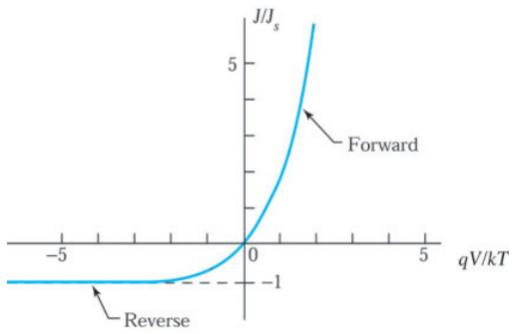
\includegraphics[width=8cm]{figures/ch01/diode_charac.jpg}
\caption{Current characteristic of equation \ref{eq:ideal_diode}}
\label{fig:diode_charac}
\end{figure}

\subsection{Caractéristique pratique de la diode}
L'équation \ref{eq:ideal_diode} donne une densité de courant. En multipliant par la surface $A$ de la section transversale de la jonction, on obtient la courbe I-V:
\begin{equation}
	i_D = I_S(e^{v_D/v_{th}} - 1)
	\label{eq:idiode_IV}
\end{equation}
avec $v_{th} = \frac{kT}{q} \approx 26 mV$ (à $T=300K$) la tension thermique (voir figure \ref{fig:diode_charac2}). Lorsque $v_D \gg v_{th}$:
\begin{equation}
	i_D \approx I_S e^{v_D/v_{th}}
\end{equation}
De plus, lorsque $v_D$ augmente d'environ $60 mV$, le courant $i_D$ est multiplié par un facteur de 10. Comme on peut le voir dans la figure \ref{fig:diode_charac2}, on peut considérer $v_D = 0,6V$ comme une tension de seuil:
\begin{itemize}
	\item Si $v_D > 0,6V$, la diode conduira,
	\item Si $v_D < 0,6V$, la diode ne conduira pas.
\end{itemize}
Ainsi, la diode fonctionne comme un redresseur: seul le courant de la région p vers la région n peut passer, tandis que l'autre direction est bloquée. Bien sûr, en raison du courant de saturation et de l'effet avalanche (voir \ref{sec:avalanche}), cela n'est pas tout à fait vrai.

\begin{figure}[h!]
\centering
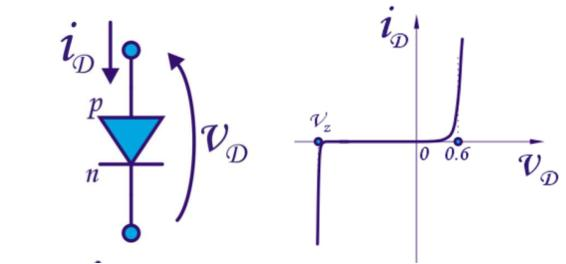
\includegraphics[width=8cm]{figures/ch01/diode_charac2.jpg}
\caption{Symbole et courbe I-V} 
\label{fig:diode_charac2}
\end{figure}

\section{Effet tunnel et avalanche}
\label{sec:avalanche}
Sur la figure \ref{fig:diode_charac2}, on peut voir qu'il y a également un point où la diode va conduire sous polarisation inverse. Ce phénomène peut avoir deux causes: soit il s'agit d'une rupture de la jonction due à l'effet avalanche, soit il s'agit d'une rupture Zener due à l'effet tunnel. La rupture de la jonction se produit à des tensions élevées et est généralement indésirable. La rupture Zener peut être utile et le dopage est adapté de manière à ce qu'elle se produise à quelques volts. Elle est utilisée, par exemple, dans les références de tension (voir le chapitre \ref{ch:references}).\\
\begin{minipage}{.5\textwidth}
	\centering
	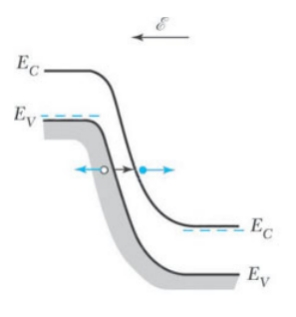
\includegraphics[height=6cm]{figures/ch01/tunnel_effect.jpg}
	\captionof{figure}{}
	\label{fig:tunnel_effect}
\end{minipage}
\begin{minipage}{.5\textwidth}
	\centering
	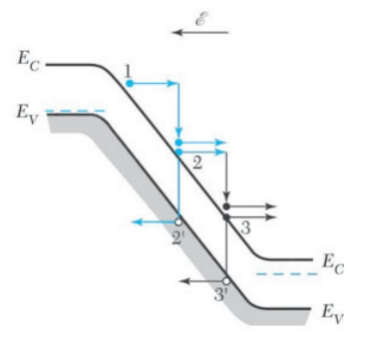
\includegraphics[width=6cm]{figures/ch01/avalanche.jpg}
	\captionof{figure}{}
	\label{fig:avalanche}
\end{minipage}\\
L'\emph{effet tunnel} repose sur la diffusion quantique : lorsque un champ électrique élevé est appliqué à une jonction p-n dans la direction inverse, comme dans la figure \ref{fig:tunnel_effect}, la distance entre la bande de valence et la bande de conduction devient localement très étroite. Dans ces circonstances, un électron de valence peut effectuer une transition de la bande de valence à la bande de conduction. Ce processus, au cours duquel un électron pénètre dans la bande interdite d'énergie, est appelé effet tunnel. L'électron et le trou résultants sont ensuite balayés par le champ électrique à travers la région de charge d'espace, ce qui crée un courant de Zener.

On parle d'\emph{effet avalanche} lorsqu'un électron généré thermiquement dans la région de charge d'espace (désignée par $1$ dans la figure \ref{fig:avalanche}) acquiert de l'énergie cinétique du champ électrique. Si le champ est suffisamment élevé, l'électron peut acquérir suffisamment d'énergie cinétique pour, lors d'une collision avec un atome, briser les liaisons du réseau, créant une paire électron-trou ($2$ et $2'$). L'électron et le trou nouvellement créés acquièrent tous deux de l'énergie cinétique du champ et créent des paires électron-trou supplémentaires (par exemple, $3$ et $3'$). Ce processus se poursuit, créant d'autres paires électron-trou. On appelle donc cette multiplication d'avalanche.

\section{Capacité de déplétion}
\label{sec:depletion_capacitance}

Lorsque nous polarisons en inverse une jonction pn, des charges positives supplémentaires apparaissent du côté n et des charges négatives supplémentaires du côté p. Ainsi, le dispositif fonctionne essentiellement comme un \emph{condensateur}. En substance, nous pouvons considérer les sections conductrices $n$ et $p$ comme les deux plaques du condensateur. Nous supposons également que la charge dans la région de déplétion réside de manière équivalente sur chaque plaque.\\
Mais ce n'est pas tout : à mesure que $V_R$ augmente, la largeur de la région de déplétion augmente également. Autrement dit, la capacité de la structure diminue à mesure que les deux plaques s'éloignent l'une de l'autre. La jonction affiche donc une capacité dépendante de la tension. Nous pouvons montrer que la capacité de la jonction $C_j$ est donnée par :
\begin{equation}
	C_j = \frac{C_{j0}}{\sqrt{1 - \frac{V_R}{V_{bi}}}}
\end{equation}
avec $C_{j0}$ la capacité à polarisation nulle ($V_R = 0$).\
Une jonction pn sous polarisation inverse est donc un condensateur contrôlable par la tension. Ce type de dispositif a de nombreuses utilisations, comme par exemple dans les circuits accordables en fréquence.

\section{Photodétecteur}
Lorsque nous polarisons une jonction pn constituée d'un semi-conducteur à bande directe comme le GaAs, nous créons un photodétecteur, comme dans la figure \ref{fig:photodetector}. Si un photon heurte un électron dans une liaison covalente, il peut rompre cette liaison si l'énergie $h \nu$ est supérieure à l'énergie de la bande interdite. La paire électron-trou résultante est ensuite balayée à travers la région de charge d'espace par le champ électrique appliqué. Ils recombinent dans les zones neutres, générant un courant proportionnel au nombre de photons qui heurtent la jonction.

\begin{figure}[h!]
	\centering
	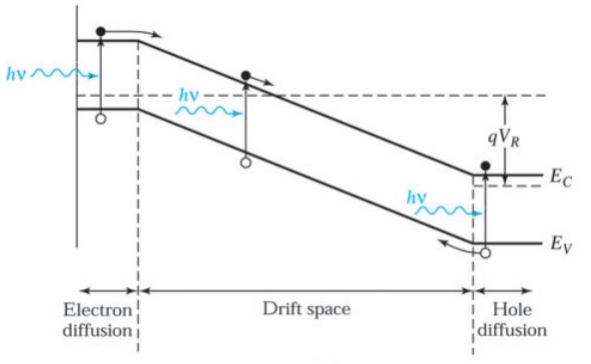
\includegraphics[width=10cm]{figures/ch01/photodetector.jpg}
	\caption{Photodetector operation} 
	\label{fig:photodetector}
\end{figure}
